To look at the free group geometrically we will consider the fundamental group on a certain kind of topological space, called a cell complex. The reader may recall that the fundamental group on a topological space comprised of certain equivalence classes of closed paths under concatenation. We will presently introduce all that we need to formally define the fundamental group.

\section{Cell Complexes}

\begin{definition}
  A \emph{complex} $K$ is a collection of \emph{simplices} of a set of vertices $V=\operatorname{Vert}(K)$; a \emph{simplex} being a collection of nonempty and finite subests of $V$. $K$ must satisfy the following.
  \begin{enumerate}
  \item If $v \in V$, we must have $\{v \} \in K$.
  \item Every nonempty subset of a simplex is also a simplex in $K$.
  \end{enumerate}
  Simplices of the form $\{ v_0, v_2, \dots v_q \}$ are said to be $q$-simplices and have \emph{dimension} $q$.
\end{definition}

\begin{definition}
  A \emph{subcomplex} $L$ of a complex $K$ is a complex with $\operatorname{Vert}(L) \subseteq \operatorname{Vert}(K)$ such that each simplex in $L$ is a simplex in $K$. We say that $L$ is \emph{full} if each simplex $s$ in $K$, such that each vertex of $s$ lies in $L$ implies that $s$ is a simplex in $L$.
\end{definition}

This is a purely algebraic representation for a topological structure. Topologically, the set the structure we defined above can be generated by the following procedure. A more detailed discussion that studies complexes from a topological point of view can be found in \cite{hatcher2002AT}.

\begin{enumerate}
\item Let $X^0 = V$ be the set of vertices or $0$-cells that is topologically discrete.
\item We create the space $X^n$ from $X^{n-1}$ inductively in the following manner. For each simplex $s$ of \emph{dimension} $n$, we suppose $e_{s}^n$ is an $n$-cell. Now as each subset of $s$ is also simplex, we have that there are a number of $n-1$-cells associated with $s$. We form $X^n$ by ``nicely'' pasting (via the disjoint union and quotient topology) the surface of each $e^n_s$ onto the $n-1$-cells associated with $s$ present in $X^{n-1}$, for each $n$-simplex $s$.
\end{enumerate}

To illustrate this, we note that $0$-simplices can be simply regarded as discrete points. A $1$-simplex of the form $\{ v_0, v_1 \}$ is associated with a line segment $[-1,1]$ where the endpoint are identified with $0$-simplices $/{v_0 /}$ and $/{v_1 /}$ which must be present in the complex by definition. A $2$-simplex of the form $\{ v_0,v_1,v_2 \}$ is associated with the circle $\bar{\mathbb{D}^2}$ that has its boundary $\mathbb{S}^1$ identified with the line segments associated with the $2$-simplices $\{ v_0,v_1 \}$, $\{ v_1,v_2 \}$ and $\{ v_2,v_0 \}$ that are necessarily present in the same complex by definition.

This disc is clearly homeomporphic to a triangle with endpoints $v_0,v_1,v_2$. In this manner, $3$-simplices can be associated with tetrahedrons that have their faces, edges and vertices associated with simplices in the complex as well, and further tetrahedrons like these compose the boundary of objects associated with $4$-simplices and so forth. Hence it makes sense to talk about the dimension of a complex which we define as follows.

\begin{definition}
  We say that the \emph{dimension} of a complex $K$ is the largest  $n \in \mathbb{N}$ such that an $n$-simplex is present in the complex or $\infty$ when there is no maximum dimension for a simplex in $K$.
\end{definition}

For reasons that will become clear when we introduce the fundamental group, we will have little need to talk about complexes of dimension greater than two. In fact our main point of interest will be in studying complexes of the following form which we will soon see are associated with free groups.

\begin{example}
  \label{exmp:bouq}
  A \emph{bouquet of $|I|$ circles} is a $1$ dimensional complex $B_I$ with $\operatorname{Vert}(B_I) = \{u_i,v_i \mid i \in I \} \cup \{ w \}$ and simplices of the form
\begin{itemize}
\item $\{ w,u_i \}$
\item $\{ w, v_i \}$
\item $\{ v_i,u_i\}$
\end{itemize}
for all $i \in I$. The topological figure associated with a bouquet of eight circles is pictured in Figure $\ref{fig:bouquet}$.
\end{example}

\begin{figure}
  \centering
  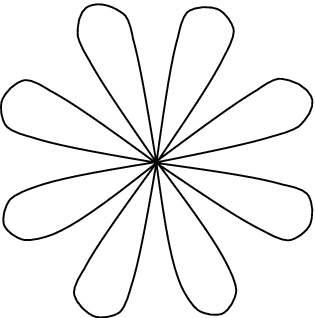
\includegraphics[scale=0.4]{bouquet.png}
  \caption{A bouquet of 8 circles}
  \label{fig:bouquet}
\end{figure}

\subsection{The Fundamental Group}
\label{sec:sc:path}

The fundamental group of a topological space $X$ based at $x_0 \in X$ is composed of homotopy classes of closed paths based at $x_0$ and its group operation is understood to be concatenation of the path classes. We will formally define the fundamental group particularly for cell complexes from an algebraic point of view, based on our definitions in the last section. Our definitions here are not conceptually different from their topological analogues, rather just describe the particular case of complexes and can be interpreted topologically keeping the topological construction from simplexes in mind. From our previous discussion we know that we can regard $2$-simplices as line segments in the complex. Giving a direction to line segments and linking these up, we have the following definitions.

\begin{definition}
  For a complex $K$, an ordered pair of vertices $\epsilon = (u,v)$ where $u$ and $v$ belong to the same simplex is called an \emph{edge} in $K$.
\end{definition}

\begin{definition}
  A \emph{path} of length $n$ from vertices $u$ to $v$ in $K$ is a sequence of $n$ edges in $K$. We denote a path $\alpha$ as follows.
  \[
    \alpha = (u,v_1)(v_1,v_2) \dots (v_{n-1},v)
  \]
  The \emph{origin} of such a path $o(\alpha) = u$ and the \emph{end} $e(\alpha) = v$. A \emph{closed} path $\alpha$ has $o(\alpha) = e(\alpha)$.

  $\alpha$ is \emph{reduced} if it is trivial or no edge $(v_i,v_{i+1})$ is adjacent to its inverse $(v_{i+1},v_i)$.
\end{definition}

\begin{definition}
  A complex $K$ is \emph{connected} if any two vertices $u,v$ of the complex are the endpoints of some path $\alpha$.
\end{definition}


A natural operation on closed paths is concatenation at the end points. It is easy to see that this operation is associative.

\begin{definition}
  If $\alpha = \epsilon_1 \dots \epsilon_n$ and $\beta = \eta_1 \dots \eta_m$ are paths in a complex $K$ with $e(\alpha) = o(\beta)$, then we define the \emph{product} $\alpha\beta$ as the concatenation of the two paths, that is
  \[
    \alpha\beta = \epsilon_1 \dots \epsilon_n\eta_1 \dots \eta_m.
  \]
\end{definition}

Now we wish to introduce a notion of homotopy in our discussion of complexes. If $K$ is a complex, note that a path comprising of two edges $(u,v)(v,w)$ can be continually morphed inside the complex $K$ to the path of one edge $(u,w)$ if the triangle with vertices $u,v,w$ is part of the $K$. This is what motivates the following notion of homotopy.

\begin{definition}
  Given a path in a complex $K$ we say that an \emph{elementary move} on this path is one of the following operations.
  \begin{itemize}
  \item If $(u,v)$ and $(v,w)$ appear as adjacent edges in a path and $\{u,v,w\}$ is a simplex in $K$, then we replace edges $(u,v)(v,w)$ in the path with the single edge $(u,w)$.
  \item If $(u,w)$ is an edge in a path, we replace it with the two edges $(u,v)(v,w)$ if $\{u,v,w\}$ is a simplex in $K$.
  \end{itemize}
  If $\alpha$ can be obtained from $\beta$ by a finite number of elementary moves, we say that $\alpha$ and $\beta$ are \emph{homotopic}, denoted $\alpha \simeq \beta$.
\end{definition}


We find that homotopy is an equivalence relation on paths in a complex $K$. That homotopy is reflexive is easy to see. For symmetry  we suppose that $\alpha \simeq \beta$. Then  $\alpha$ can be produced from $\beta$ by applying the inverses of the elementary moves required to go from $\alpha$ to $\beta$ in reverse order. 

For transitivity, we suppose $\alpha \simeq \beta$ and $\beta \simeq \gamma$. Then $\alpha \simeq \gamma$ by applying the finitely many elementary moves to go from $\alpha$ to $\beta$ followed by the finitely many required to go from $\beta$ to $\gamma$.

In topological complexes, every path is homotopic to a path that is a sequence of edges. This homotopy is achieved by morphing the path to stick to the boundary of every $n$-cell it is on till it sticks to $1$-cells only. Then we may ``smooth'' out the path by removing partial traversals down an edge and shrink the ends till the endpoints meet the nearest vertices. The resultant path then comprises of a sequence of edges. What this means that the homotopy classes of paths defined simplically can be exactly associated with their topological analogues, even if the paths themselves cannot.

\begin{definition}
  We say that the equivalence class of paths homotopic to $\alpha$ is its \emph{path class} $[\alpha]$. Endpoints of paths in $[\alpha]$ must remain constant and we denote them $o[\alpha]$, $e[\alpha]$ for the origin and end respectively
\end{definition}

The product of path classes is taken to be $[\alpha][\beta] = [\alpha\beta]$ and is well defined when $e[\alpha] = o[\beta]$. To see this, consider $\alpha' \in [\alpha]$ and $\beta' \in [\beta]$. Since $\alpha', \beta'$ are produced by applying finitely many elementary moves on $\alpha,\beta$ respectively, we can these apply these moves together on $\alpha\beta$ to produce $\alpha'\beta'$. Thus $[\alpha'] = [\alpha]$ and $[\beta'] = [\beta]$ implies that $[\alpha'\beta'] = [\alpha\beta]$ as required.

This operation on the set of closed path classes is easily shown to be associative. The stationary path composed of no edges forms the path class $[(u,u)]$ has that $[\alpha][(u,u)] = [(u,u)][\alpha] = [\alpha]$ for all closed path classes $[\alpha]$. Lastly we notice that if $[\alpha]$ is a closed path class with $\alpha=(u,v_1)(v_1,v_2) \dots (v_n,u)$ we have that $\bar{\alpha}=(u,v_n)(v_n,v_{n-1}) \dots (v_1,u)$ has $[\alpha][\bar{\alpha}] = [\bar{\alpha}][\alpha] = [(u,u)]$. Thus we have satisfied all the group axioms.

\begin{definition}
  For a complex $K$ and some vertex $v$ called the \emph{basepoint}. The \emph{fundamental group} of a $K$ with respect to $v$ is the set
  \[
    \pi(K,v) = \{[\alpha]: o[\alpha] = e[\alpha] = v \}
  \]
  under multiplication of path classes.
\end{definition}

Note that if $K$ is a connected complex, then for any two vertices $u,v$ that $\pi(K,u) \cong \pi(K,v)$. To see this, we use the fact that there is a path $\alpha$ with endpoints $u$ and $v$. It is then possible to show that $\phi : \pi(K,u) \rightarrow \pi(K,v)$ given by $[\gamma] \mapsto [\bar{\alpha} \gamma \alpha]$ is well defined and an isomorphism. 
Consequently, we may omit referring to a basepoint when talking about the fundamental group of connected complexes.

We also find that some kinds of maps between complexes correspond to homomorphisms between their fundamental group. We define the following, analogous to continuous maps between complexes thought of topologically.

\begin{definition}
  A simplical map $\phi:K \rightarrow L$ where $K,L$ are complexes is a map that sends each vertex $v \in \operatorname{Vert}(K)$ in a simplex to $\phi v$ such that when $\{ v_0, v_1, \dots v_n \}$ is a simplex in $K$, $\{\phi v_0, \phi v_1, \dots \phi v_n\}$ is a simplex in $L$. If $\phi:K \rightarrow L$ is simplical and invertible with $\phi^{-1}$ also simplical, we say that $\phi$ is an isomorphism (cf. homeomorphisms).
\end{definition}

The following is easy to prove for simplical complexes and is a standard result for continuous maps on topological spaces. For a simplical map $\phi:K \rightarrow L$, if $\alpha = (u,v_1)(v_1,v_2) \dots (v_n,v)$ is a path in a complex $K$, then $(\phi u,\phi v_1)(\phi v_1,\phi v_2) \dots (\phi v_n,\phi v)$ is a path in $L$ that we call $\phi \alpha$

\begin{theorem}
  If $\phi:K \rightarrow L$ is a simplical map and $v \in \operatorname{Vert}(K)$, then there exists a homomorphism $\phi_{\#}:\pi(K,v) \rightarrow \pi(L,\phi v)$ defined by $[\alpha] \mapsto [\phi \alpha]$.
\end{theorem}

\begin{proof}
Omit.  
\end{proof}

\begin{definition}
  A \emph{tree} in $K$ is a subcomplex $T$ of dimension no greater than $1$ with no reduced closed paths and is \emph{maximal} if $T$ is contained in no larger tree in $K$.
\end{definition}

\begin{definition}
  If $T$ is a maximal tree in a connected complex $K$, then $\mathcal{T}(K,T)$ is the group having the presentation with generators comprised of all edges in $K$ and relations comprised of the following types.
  \begin{itemize}
  \item $(u,v) = 1$ if $(u,v)$ is an edge in $T$;
  \item $(u,v)(v,x)$ = $(u,x)$ if $\{u,v,x \}$ is a simplex in $K$.
  \end{itemize}
\end{definition}

The following theorem will be key in bringing free groups into our discussion of complexes.

\begin{theorem}[Tietze's]
  If $K$ is a connected complex and $T$ is a maximal tree in $K$, then
  \[
    \pi(K,w) \cong \mathcal{T}(K,T).
  \]
\end{theorem}

\begin{proof}
  Let $X$ be the set of all edges $(u,v)$; that is where $u,v \in \operatorname{Vert}(K)$ and $\{ u,v \}$ is a distinct simplex in $K$ (allows for multiple edges between the same two points). This is by definition the set of generators of $\mathcal{T}(K,T)$. Let $R$ be the normal subgroup generated by the set of relations on $\mathcal{T}(K,T)$, i.e.\ edges in $T$ and the words $(u,v)(v,x)(u,v)^{-1}$ when $\{u,v,x \}$ is a simplex in $K$.

  Now suppose that $F$ is the free group generated by $X$. By definition $\mathcal{T}(K,T) = F/R$. Let $w \in \operatorname{Vert}(K)$ and define
  \begin{itemize}
  \item For $v \in \operatorname{Vert}(K) - \{w\}$, the unique reduced path between $w$ and $v$ in $T$ to be $\lambda_v$. This exists since $T$ is a maximal tree;
  \item $\lambda_w$ to be the trivial path $(w,w)$.
  \end{itemize}

Now define a function $f:X \rightarrow \pi(K,w)$ by
\begin{equation*}
  (u,v) \mapsto [\lambda_u(u,v)\lambda_v^{-1}].
\end{equation*}

Since $F$ is free, there is a unique homomorphism $\phi: F \rightarrow \pi(K,w)$. We claim that $R \leq \ker \phi$. To see this, we consider the two types of words in $R$.
\begin{itemize}
\item If $(u,v)$ is an edge in $T$, then $\lambda_u (u,v) \lambda_v^{-1}$ is a path in $T$ \emph{based} at $w$. However, $T$ is a tree with no circuits and hence $\lambda_u (u,v) \lambda_v^{-1}$ must be the trivial path $(w,w)$ after reducing. Therefore $[\lambda_u (u,v) \lambda_v^{-1}]$ is the identity in $\pi(K,w)$.
\item If $\alpha = (u,v)(v,x)(u,x)^{-1}$ is a path with the simplex $\{ u,v,x \}$ present in $K$, then we have the following.
  \begin{align*}
    [\lambda_u (u,v) \lambda_v^{-1}][\lambda_v (v,x) \lambda_x^{-1}] &= [\lambda_u (u,v) \lambda_v^{-1}\lambda_v (v,x) \lambda_x^{-1}] \\
                                                                     &= [\lambda_u (u,v)(v,x) \lambda_x^{-1}] \\
                                                                     &= [\lambda_u (u,x) \lambda_x^{-1}]. \\
  \end{align*}
  Thus $\phi((u,v))\phi((v,x)) = [\lambda_u (u,v) \lambda_v^{-1}][\lambda_v (v,x) \lambda_x^{-1}] = [\lambda_u (u,x) \lambda_x^{-1}] = \phi((u,x))$ in $\pi(K,w)$. It follows that $\phi(\alpha) = [(w,w)]$ as required.
\end{itemize}
Since $R$ is the smallest normal subgroup containing elements of these types, it must be contained in $\ker \phi$.

Since $\mathcal{T}(K,T) = F/R$, there must be a homomorphism $\Phi: \mathcal{T}(K,T) \rightarrow \pi(K,w)$ given by

\begin{equation*}
  (u,v)R \mapsto [\lambda_u (u,v) \lambda_v^{-1}].
\end{equation*}

In fact, the following diagram with $\Phi$ commutes.

\begin{equation*}
  \begin{tikzcd}[ampersand replacement=\&, sep=huge]
    \mathcal{T}(K,T) \arrow[dr,dashrightarrow,"\Phi"] \\
    F \arrow[u,twoheadrightarrow] \arrow[r,"\phi"] \& \pi(K,w).
  \end{tikzcd}
\end{equation*}

We claim that $\Phi$ is in fact an isomorphism and prove this by showing that it is invertible. Let $\alpha = \epsilon_1 \epsilon_2 \dots \epsilon_n$ be a closed path in $K$ at $w$ with each $\epsilon_i$ being an edge. Let

\begin{equation*}
\theta(\alpha) = \alpha R \in \mathcal{T}(K,T).
\end{equation*}

If $\beta$ is homotopic to $\alpha$ then the relations of $\mathcal{T}(K,T)$ show that $\theta(\alpha) = \theta(\beta)$. Thus the function $\Theta:\pi(K,w) \rightarrow \mathcal{T}(K,T)$ given by $[\alpha] \mapsto \theta(\alpha)$ is well defined and easily seen to be a homomorphism. However,

\begin{align*}
  \Phi(\alpha R) &= \Phi(\epsilon_1 \epsilon_2 \dots \epsilon_n R) \\
                 &= \Phi(\epsilon_1 R) \Phi(\epsilon_2 R) \dots \Phi(\epsilon_n R) \\
                 &= [\lambda_w \epsilon_1 \lambda_{v_1}^{-1}]  \dots [\lambda_{v_{n-1}}\epsilon_n \lambda_w^{-1}] \\
                 &= [\lambda_w\epsilon_1 \epsilon_2 \dots \epsilon_n \lambda_w^{-1}] \\
                 &= [\epsilon_1 \epsilon_2 \dots \epsilon_n] \\
                 &= [\alpha].
\end{align*}
Since $\lambda_w$ is trivial. In particular, $\Phi\Theta([\alpha]) = [\alpha]$ and $\Phi\Theta$ must be the identity map on $\pi(K,w)$. On the other hand, for an edge $(u,v)$ in $K$,
\begin{align*}
  \Theta\Phi((u,v) R) &= \Theta(\phi(u,v)) \\
                      &= \Theta([\lambda_u(u,v)\lambda_v^{-1}])
                      &= \lambda_u (u,v) \lambda_v^{-1} R.
\end{align*}
Since $\lambda_v$ is a path in $T$, it follows that each of its edges lie in $T$ and thus in $R$. Consequently the last term above simplifies to $\lambda_u(u,v)R$. By the same reasoning, $\lambda_u$ also lies in $R$ and by the normality of $R$ we can further simplify it to $(u,v) R$. Since the generators of $\mathcal{T}(K,T)$ have that $\Theta\Phi$ is the identity on them, we must have that $\Theta\Phi$ is the identity on the whole $\mathcal{T}(K,T)$. Hence $\Phi: \mathcal{T}(K,T) \rightarrow \pi(K,w)$ is an isomorphism as required.
\end{proof}

When we limit our discussion to complexes of dimension $1$, we have the following corollary.

\begin{corollary}
  \label{cor:1free}
  If $K$ is a connectd $1$-complex, then $\pi(K,w)$ is a free group for some $w \in \operatorname{Vert}(K)$ with
  \begin{equation*}
    \operatorname{rank} \pi(K,w) = |\{1 \text{-simplexes in } K \text{ not in } T \}|.
  \end{equation*}
\end{corollary}

\begin{proof}
  By the theorem we have that $\pi(K,w)$ is isomorphic to $\mathcal{T}(K,T)$, where $T$ is a maximal tree of $K$. This has generators composed of all edges in $K$.

  If $(u,v) \in T$ then $(u,v) \in R$, so we can delete these generators and remove it from the relations altogether. Since the complex is of dimension $1$, relations of the second type do not exist and the subgroup of relations we are left with only has only the identity. Thus $\mathcal{T}(K,T)$ is the free group with the set of generators being $\{(u,v) \{1\} \mid (u,v) \text{ is an edge not in } T\}$. Since $(v,u) \{1\} = (u,v)^{1} \{ 1 \}$ we need include only one of $(u,v)$ or $(v,u)$ as a generator since the other would appear by the definition of the free group. Now our remaining generators correspond exactly to $1$-simplices in $K$ that are not in $T$.
\end{proof}


\begin{example}
  \label{exmp:bouq-fund}
  If $B_I$ is the bouquet of $|I|$ circles as in Example \ref{exmp:bouq}, then $\pi(B_I,w) \cong F_{|I|}$. We define $T = \{ \{w,u_i \} | i \in I \} \cup \{ \{w,v_i \} | i \in I \}$ and notice that this is a maximal tree. The remaining simplices are $\{v_i,u_i\}$, of which there are exactly $|I|$ of. The corollary above then gives us that $\pi(B_I,w)$ is free with rank $|I|$ as required.
\end{example}

\section{Covering Complexes}
We will now turn our attention to covering complexes. Given a simplical complex, we find that there exist ``larger'' complexes that locally appear similar to the simplical complex. We will see that the fundemental groups of these are bear relations to the fundamental group of the complex that they ``cover''.

\begin{definition}
  Let $K$ and $K'$ be complexes and suppose $p: K \rightarrow K'$ is a simplical map. We say that for a subcomplex $L'$ of $K'$, the \emph{inverse image} of $L'$ is defined to be
  \begin{equation*}
    p^{-1}(L') = \{ \text{simplices } s \in K \mid p(s) \in L' \}.
  \end{equation*}
\end{definition}

Firstly we note that $p^{-1}(L')$ must indeed be a subcomplex of $K$. To see this we need to check that the collection of simplices in $p^{-1}(L')$ satisfy the definition.

\begin{itemize}
\item Suppose that $v$ is a vertex in $p^{-1}(L')$. Then we must have that $v$ belongs to a simplex in $p^{-1}(L')$; in particular there must exist a simplex $s \in K$ that at contains $v$ and has that $p(s) \in L'$. However, by the definition of the simplical map, $p$ acts uniformly on vertices. Therefore, since $p(s)$ is a simplex in $L'$ that contains $p(v)$, $\{ p(v) \} = p(\{ v \})$ is also a simplex in $L'$ and so $\{ v \} \in p^{-1}(L')$.
\item Suppose $s$ is a simplex in $p^{-1}(L')$ and so $p(s) \in L'$. Now each subset of $r \subseteq s$ is also a simplex in $K$ with $p(r) \subseteq p(s)$. In particular, $p(r)$ must be a simplex in $L'$ and it follows that $r$ is a simplex in $p^{-1}(L')$.
\end{itemize}

Let us denote for a simplex $s$ in $K$, the set of all nonempty subsets of $s$ by $|s|$. We notice that if $s \in K'$, then since $|s|$ can be considered a subcomplex, we have that $p^{-1}(|s|)$ is a subcomplex of $K$. What follows is that if $L'$ is a full subcomplex of $K'$, then we must have that $p^{-1}(L')$ too is a full subcomplex of $K'$.
\begin{definition}
  Let $K$ be a complex. We say that a \emph{covering complex} $\tilde{K}$  of $K$ is a connected complex such that there is a simplical map $p:\tilde{K} \rightarrow K$ such that for each simplex $s \in K$, we can write
  \begin{equation*}
    p^{-1}(|s|) = \bigcup_{i \in I} |\tilde{s_i}|
  \end{equation*}
  For an indexing set $I$ and such that $|\tilde{s_j}|$ and $|\tilde{s_k}|$, each $\tilde{s_i}$ being a simplex of $\tilde{K}$, are disjoint when $j \neq k$. Further we must have that the restrictions $p \vert_{|\tilde{s_i}|} : |\tilde{s_i}| \rightarrow |s|$, called the \emph{projection}, is an isomorphism for each $i \in I$. The subcomplexes $|\tilde{s_i}|$ from above are called the \emph{sheets} over $s$.
\end{definition}

Covering complexes, or covers, are the notion of ``larger'' complexes that we alluded to in the introduction to this section. An important result in algebraic topology gives us a one-to-one correspondence between covers of any topological space and the subgroups of the fundamental group of this topological space. In the rest of this section we will show this in the less general case of simplical complexes, which is all we are concerned with for our discussion of free groups.

\begin{theorem}
  Let $p:\tilde{K} \rightarrow K$ be a covering complex and suppose that $\tilde{w}$ is a vertex in $\tilde{K}$ with $p(\tilde{w}) = w$ for some point $w \in K$. Then, for any path $\alpha$ in $K$ with $o(\alpha) = w$ there exists a \emph{unique} path $\tilde{\alpha}$ in $\tilde{K}$ such that $o(\tilde{\alpha}) = \tilde{w}$ and $p\tilde{\alpha} = \alpha$. We call this unique path $\tilde{\alpha}$ the \emph{lifting} of $\alpha$.
\end{theorem}

\begin{proof}
  Recall that the length of a path is the number of edges it has, which is necessarily finite. Thus we show that the theorem holds for a path of each length $n \in \mathbb{N}$ by induction.

  For $n=1$, without loss of generality, we can suppose that $\alpha = (w,u)$ for some endpoint $u \in K$ where $u$ belongs to a simplex that $w$ does. Thus $s = \{ w,u \}$ is a $1$-simplex in $K$. Let $|\tilde{s}|$ be the sheet over $|s|$ that contains $\tilde{w}$ then since $p \vert_{|\tilde{s}|}$ is an isomorphism, $\{ \tilde{w}, \tilde{u}\}$ is a $1$-simplex in this sheet and so $(\tilde{w},\tilde{u})$ is an edge with $p(\tilde{w},\tilde{u})=(w,u)$. Now we need to show that $(\tilde{w}, \tilde{u})$ is unique. For this suppose that $(\tilde{w}, \tilde{v})$ is also a lifting and so $\{ \tilde{w}, \tilde{v} \}$ is a $1$-simplex in $\tilde{K}$. It follows that $(\tilde{w}, \tilde{v})$ is also a sheet over $\{ w,u \}$ but $\{w\} \in |\{\tilde{w}, \tilde{u}\}| \cap |\{\tilde{w}, \tilde{v}\}|$ which contradicts the definition of the covering complexes (sheets must be disjoint) and it follows that $\tilde{u} = \tilde{v}$.

  Suppose now that $n>1$, and that the theorem holds for all paths of length less than $n$. Then each path $\alpha$ in $K$ of length $n$ can be written as $(w,u)\beta$ where $\beta$ is a path of length $n-1$ with origin at $u$. We know that there are unique liftings of $(w,u)$ and $\beta$ to $(\tilde{w},\tilde{u})$ and $\tilde{\beta}$ respectively where the origin of $\tilde{\beta}$ is $\tilde{u}$. Thus $\tilde{\alpha} = (\tilde{w},\tilde{u})\tilde{\beta}$ is the unique lifting of $\alpha$.
\end{proof}

What this theorem shows is that for the index $I$ of a path $\alpha$ in $K$ that there exists a path $\tilde{\alpha}$ in $\tilde{K}$ also indexed by $I$ such that the following diagram commutes. Furthermore for a fixed basepoint $\tilde{w}$ as the origin of $\tilde{\alpha}$, this path is unique.


\begin{equation*}
    \begin{tikzcd}[ampersand replacement=\&, sep=huge]
      \& \tilde{K} \arrow[d,"p"] \\
    I \arrow[ur,dashrightarrow,"\tilde{\alpha}"] \arrow[r,"\alpha"] \& K
  \end{tikzcd}
\end{equation*}

\begin{lemma}
  \label{lem:lift-homo}
  Let $p:\tilde{K} \rightarrow K$ be a covering complex, and suppose $\tilde{w}$ is a vertex in $\tilde{K}$ with $p(\tilde{w}) = w $ for some $w \in \operatorname{Vert}(K)$. Then if $\alpha$ and $\beta$ are homotopic in $K$ with origins $w$, we have that their liftings $\tilde{\alpha}$ and $\tilde{\beta}$ with origins at $\tilde{w}$ are homotopic with $e(\tilde{\alpha}) = e(\tilde{\beta})$.
\end{lemma}

\begin{proof}
  Let $\tilde{u},\tilde{v},\tilde{x}$ be vertices of $\tilde{K}$ such that $(\tilde{u},\tilde{v})(\tilde{v},\tilde{x})$ is a lifting of $(u,v)(v,x)$ where $\{u,v,x\} = s$ is  simplex in $K$. If $\tilde{s}$ the sheet over $s$ that contains $\tilde{v}$ we know that it is isomorphic to $s$ so has the form $\{\tilde{v}, \tilde{u}', \tilde{x}' \}$ where $\tilde{u}'$ and $\tilde{x}'$ are vertices in $\tilde{K}$. Similarly $\tilde{t}$, the sheet over $s$ containing $\tilde{u}$ can be written $\{\tilde{u},\tilde{v}'',\tilde{x}''\}$ where $\tilde{v}'',\tilde{x}'' \in \operatorname{Vert}{\tilde{K}}$. Now by the definition of sheets and without loss of generality we can assume that $p\tilde{v}'' = v$, $p\tilde{u}' = u$ and $p\tilde{x}' = p\tilde{x}'' = x$. It follows that $(\tilde{u},\tilde{v})$ and $(\tilde{u},\tilde{v}'')$ are liftings of $(u,v)$ but have the same origin and by uniqueness of lifting up to origin they must be the same and we have $\tilde{v} = \tilde{v}''$. Now, by the fact that sheets must be disjoint, we must have that $\tilde{s} = \tilde{t}$ therefore $\tilde{u} = \tilde{u}'$ and $\tilde{x}' = \tilde{x}''$ as well. This argument can be repeated for the edge $(\tilde{v},\tilde{x})$ to show that $\tilde{x} = \tilde{x}'$ and thus $\tilde{s} = \{\tilde{u},\tilde{v},\tilde{x}\}$ is a simplex in $\tilde{K}$.

  It follows that the elementary moves applied to $\alpha$ in $K$ can be analogously applied to $\tilde{\alpha}$ and if $\alpha'$ is acquired after applying an elementary move to $\alpha$, the lift of $\alpha'$ is equal to the analogous elementary move being applied to $\tilde{\alpha}$. In particular when $\alpha \simeq \beta$, applying the analogous finitely elementary moves to $\tilde{\alpha}$ gives us that $\tilde{\alpha} \simeq \tilde{\beta}$. Furthermore, since elementary moves do not affect the endpoints of paths, we have that $e(\tilde{\alpha}) = e(\tilde{\beta})$.
\end{proof}

\begin{theorem}
  \label{thm:injection}
  Let $p:\tilde{K} \rightarrow K$ be a covering of a complex $K$ and $\tilde{w} \in \operatorname{Vert}(\tilde{K})$ such that for some vertex $w$ of $K$, $p(\tilde{w}) = w$. Then considering $\tilde{w}$ a basepoint of $\tilde{K}$ and $w$ of $K$, we have that the induced homomorphism $p_{\#} : \pi(\tilde{K},\tilde{w}) \rightarrow \pi(K,w)$ is injective.
\end{theorem}

\begin{proof}
  Suppose $[\tilde{\alpha}],[\tilde{\beta}] \in \pi(\tilde{K},\tilde{w})$ with $p_{\#}[\tilde{\alpha}] = p_{\#}[\tilde{\beta}]$; equivalently $p\tilde{\alpha} \simeq p\tilde{\beta}$. But $\tilde{\alpha}$ and $\tilde{\beta}$ are the liftings of $p\tilde{\alpha}$ and $p\tilde{\beta}$ respectively at basepoint $\tilde{w}$ and Lemma \ref{lem:lift-homo} asserts that they are homotopic. Thus $\tilde{\alpha} \simeq \tilde{\beta}$ and hence $[\tilde{\alpha}] = [\tilde{\beta}]$.
\end{proof}

\begin{theorem}
  \label{thm:conj}
  Let $p: \tilde{K} \rightarrow K$ be a covering complex and suppose $\tilde{w}$ is a basepoint in $\tilde{K}$ with $p(\tilde{w}) := w \in K$. If another vertex $\tilde{u}$ in $\tilde{K}$ has $p(\tilde{u}) = w$, then $p_{\#}\pi(\tilde{K},\tilde{w})$ and $p_{\#}\pi(\tilde{K},\tilde{u})$ are conjugate subgroups of $\pi(K,w)$. Conversely If $H \leq \pi(K,w)$ is conjugate to $p_{\#}\pi(\tilde{K},\tilde{w})$, then there exists a vertex $\tilde{u} \in \tilde{K}$ with $p(\tilde{u}) = w$ such that $H = p_{\#}\pi(\tilde{K},\tilde{u})$.
\end{theorem}

\begin{proof}
  By the definition of covering complexes $\tilde{K}$ is connected and there must be a path $B$ in $\tilde{K}$ with $o(B) = \tilde{w}$ and $e(B) = \tilde{u}$. From how we've defined $\tilde{w}$ and $\tilde{u}$ the path $\beta:=pB$ must be closed and based at $w$, and thus $[\beta] \in \pi(K,w)$. We will show that
  \begin{equation}
    \label{eq:conjugate}
    [\beta]^{-1} p_{\#}\pi(\tilde{K},\tilde{w}) [\beta] = p_{\#}\pi(\tilde{K},\tilde{u}).
  \end{equation}
  If $[\alpha]$ is a path class in $p_{\#}\pi(\tilde{K},\tilde{w})$ such that $\alpha$ lifts to $\tilde{\alpha}$ at $\tilde{w}$, then $\tilde{\alpha}$ is a closed path based at $\tilde{w}$ and $B^{-1} \tilde{\alpha} B$ is a closed path based at $\tilde{u}$ which means that $[B^{-1} \tilde{\alpha} B] \in \pi(\tilde{K},\tilde{u})$. It is easy to check that $p(B^{-1} \tilde{\alpha} B) = \beta^{-1}\alpha\beta$ and so
  \begin{equation*}
    p_{\#}[B^{-1} \tilde{\alpha} B] = [p(B^{-1} \tilde{\alpha} B)] = [\beta^{-1}\alpha\beta] = [\beta^{-1}][\alpha][\beta].
  \end{equation*}
  Thus $[\beta^{-1}][\alpha][\beta] \in p_{\#}\pi(\tilde{K},\tilde{u})$ for all $[\alpha] \in p_{\#}\pi(\tilde{K},\tilde{w})$. An identical argument can be applied to path classes of $p_{\#}\pi(\tilde{K},\tilde{u})$ to show that $[\beta] p_{\#}\pi(\tilde{K},\tilde{u}) [\beta]^{-1} \subseteq p_{\#}\pi(\tilde{K},\tilde{w})$ from which our claim of equation \ref{eq:conjugate} is verified.

  For the converse part of the theorem, suppose that $H = [\alpha]p_{\#}\pi(\tilde{K},\tilde{w})[\alpha]^{-1}$ and that $\tilde{\beta}$ is  the unique lifting of $\alpha^{-1}$ in $\tilde{K}$ with origin $\tilde{w}$. We set $\tilde{u}$ as the endpoint of $\tilde{\beta}$, then $p(\tilde{u}) = w$ since $w$ is the endpoint of $\alpha^{-1}$. Now by definition $[\gamma] \in H$ if and only if $[\alpha^{-1}\gamma\alpha] \in p_{\#}\pi(\tilde{K},\tilde{w})$. This is equivalent to there being a lifting of $\alpha^{-1} \gamma \alpha$ at $\tilde{w}$. But the lifting must be $\tilde{\beta} \tilde{\gamma} \tilde{\beta}^{-1}$ for some path $\tilde{\gamma}$ in $\tilde{K}$. However, considering the endpoints of $\tilde{\beta}$, we must have that $\tilde{\gamma}$ is a closed path at $\tilde{u}$ and so $\gamma$ lifts to $\tilde{\gamma}$ at $\tilde{u}$, equivalent to $[\gamma] \in p_{\#}\pi(\tilde{K},\tilde{u})$. The reverse of this argument can be run and we have that $H = p_{\#}\pi(\tilde{K},\tilde{u})$.
\end{proof}

With this, we establish some relation between the coverings of a complex and the subgroups of its fundamental groups. In particular, since the induced homomorphism is injective, the fundamental groups of covers are all isomorphic to one another as well as to some subgroups of the fundamental group of the complex that are conjugate.

It is clear in the proofs that we have seen that the preimage of a vertex $w$ in the covering map has some significance, i.e.\ which paths can paths based at $w$ lift to. For this we define the following.


\begin{definition}
  If $p:\tilde{K} \rightarrow K$ is a simplical map and $w$ is a vertex in $K$, then we say that the \emph{fiber} over $w$ is the set $p^{-1}(w)$.
\end{definition}

\begin{theorem}
  Let $p:\tilde{K} \rightarrow K$ be a covering complex and suppose $w$ is a vertex in $K$. Then $\pi(K,w)$ acts on $p^{-1}(w)$ transitively by
  \begin{equation*}
    {\tilde{w}}\cdot[\alpha] = e[\tilde{\alpha}]
  \end{equation*}
  for each $\tilde{w} \in p^{-1}(w)$. The action has stabiliser $p_{\#}\pi(\tilde{K},\tilde{w})$ for the point $\tilde{w} \in p^{-1}(w)$.
\end{theorem}

\begin{proof}
  First, note that the action is well defined for the following reasons.
  \begin{itemize}
  \item Lemma \ref{lem:lift-homo} gives us that homotopic paths lift to homotopic paths with the same endpoint. Thus our choice of path in $[\alpha]$ doesn't change the endpoint of its lifting for a given basepoint.
  \item The endpoint of $\tilde{\alpha}$ is mapped to $w$ by $p$ since that is the endpoint of $\alpha$.
  \end{itemize}
  
  Now we will check that this is indeed a group action. The identity in $\pi(K,w)$ is $[(w,w)]$ and for basepoint $\tilde{x} \in p^{-1}(w)$, the path $(w,w)$ lifts to $(\tilde{x},\tilde{x})$ which has $\tilde{x}$ as its endpoint as required.

  Next suppose that $[\alpha]$ and $[\beta]$ are path classes in $\pi(K,w)$ and let $\tilde{x} \in p^{-1}(w)$. Let $\tilde{\alpha}$ be the lifting of $\alpha$ and at basepoint $\tilde{x}$ and if $\tilde{y}$ is the endpoint of $\tilde{\alpha}$, let $\tilde{\beta}$ be the lifting of $\beta$ at basepoint $\tilde{y}$; It is easy to see that $\tilde{\alpha}\tilde{\beta}$ is the lifting of the path $\alpha\beta$ at $\tilde{x}$. We have thus that
  \begin{equation*}
    \tilde{x}[\alpha\beta] = e[\tilde{\alpha}\tilde{\beta}] = e[\tilde{\beta}] = \tilde{y}[\beta] = (e[\tilde{\alpha}])[\beta] = \tilde{x}[\alpha][\beta]
  \end{equation*}
  by the uniqueness of liftings at a basepoint.

  To see that the action is transitive, let $\tilde{x}$ and $\tilde{y}$ be elements of the fiber $p^{-1}(w)$ and by the connectedness of $\tilde{K}$, let $A$ be a path from $\tilde{x}$ to $\tilde{y}$. Let $\alpha$ be the path based at $w$ such that $pA = \alpha$ so $[\alpha] \in \pi(K,w)$. We have then that
  \begin{equation*}
    \tilde{x}[\alpha] = e[A] = \tilde{y}.
  \end{equation*}

  Lastly, we check that the stabiliser of the action at a point $\tilde{x} \in p^{-1}(w)$ is indeed $p_{\#}\pi(\tilde{K},\tilde{x})$. $[\alpha]$ belongs to the stabiliser of $\tilde{x}$ if and only if it lifts to closed paths at $\tilde{x}$ which happens if and only if $[\alpha] \in p_{\#}\pi(\tilde{K},\tilde{x})$.
\end{proof}

\begin{corollary}
  Let $p: \tilde{K} \rightarrow K$ be a covering complex. Then we have the following.
  \begin{enumerate}
  \item If $w$ is a basepoint in $K$ and $\tilde{w} \in p^{-1}(w)$, then
    \begin{equation*}
      [\pi(K,w) : p_{\#}\pi(\tilde{K},\tilde{w})] = |p^{-1}(w)|.
    \end{equation*}
  \item If $w,u$ are basepoints in $K$, then
    \begin{equation*}
      |p^{-1}(w)| = |p^{-1}(u)|.
    \end{equation*}
  \end{enumerate}
\end{corollary}

\begin{proof}
  \begin{enumerate}
  \item The cardinality of a set with a transitive action defined on it is the index of the stabiliser at a point.
  \item If $w$ and $u$ are basepoints in $K$, there is are isomorphisms $\phi,\psi$ on $\pi(K,w)\rightarrow\pi(K,u)$ and $\pi(\tilde{K},\tilde{w})\rightarrow\pi(\tilde{K},\tilde{w})$ respectively. We will not show this here but it follows a similar line of reasoning to that seen in the proof of Theorem \ref{thm:conj}. It can be shown then that the following diagram commutes and the result follows.
    \begin{equation*}
      \begin{tikzcd}[ampersand replacement=\&, sep=huge]
        \pi(\tilde{K},\tilde{w})\arrow[r,"\phi"]\arrow[d,"p_{\#}"]\& \pi(\tilde{K},\tilde{u}) \arrow[d,"p_{\#}"] \\
        \pi(K,w) \arrow[r,"\psi"] \& \pi(K,u)
      \end{tikzcd}
    \end{equation*}
  \end{enumerate}
\end{proof}

\begin{definition}
  Let $K$ be a complex with basepoint $w$ and suppose $\pi \leq \pi(K,w)$. We define the following relation on paths with origin $w$
  \begin{equation*}
    \alpha \equiv_\pi \beta \quad\text{if}\qquad e(\alpha) = e(\beta) \quad\text{and}\quad [\alpha\beta^{-1}] \in \pi.
  \end{equation*}
\end{definition}

To see that $\equiv_{\pi}$ is an equivalence relation, we check the following. Let $\alpha,\beta,\gamma$ be paths originating at $w$;
\begin{enumerate}
\item Trivially, $e(\alpha) = e(\alpha)$ and $[\alpha \alpha^{-1}] = [(w,w)]$ which belongs to every subgroup of $\pi(K,w)$.
\item If $\alpha \equiv_{\pi} \beta$, then $e(\beta) = e(\alpha)$ and $[\alpha \beta^{-1}] = [(\beta \alpha^{-1})^{-1}] \in \pi$. It follows by the definition of the subgroup that $[\beta \alpha^{-1}] \in \pi$ and hence $\beta \equiv_{\pi} \alpha$.
\item Lastly suppose $\alpha \equiv_{\pi} \beta$ and $\beta \equiv_{\pi} \gamma$. Then $\alpha,\beta,\gamma$ must all have the same endpoint with $[\alpha\beta^{-1}],[\beta\gamma^{-1}] \in \pi$ and so $[\alpha\beta^{-1}][\beta\gamma^{-1}] = [\alpha\gamma^{-1}]$ also belongs to $\pi$. It follows that $\alpha \equiv_{\pi} \gamma$ as required.
\end{enumerate}

Let \emph{$\mathcal{C}\alpha$} denote the equivalence class under $\equiv_{\pi}$ that the path $\alpha$ belongs to and suppose that $K_{\pi}$ is the set of all such equivalence classes for a subgroup $\pi \leq \pi(K,w)$. We find that we can consider $K_{\pi}$ as a complex in the following way.

Let $s$ be a simplex in $K$ and suppose $\alpha$ is a path in $K$ with origin at the basepoint $w$ and has its endpoint as a vertex in simplex $s$. We say that a \emph{continuation} of $\alpha$ in $s$ is a path $\beta = \alpha\alpha'$, for a path $\alpha'$ that lies completely in $s$. Now, we say that the simplices of $K_{\pi}$ are sets of the form
\begin{equation*}
  [s,\mathcal{C}\alpha] := \{\mathcal{C}\beta \mid \beta \text{ is a continuation of } \alpha \text{ in } s \},
\end{equation*}
For a simplex $s$ of $K$ and any path $\alpha$ originating from $w$ in $K$. In particular the equivalence classes in $[s,\mathcal{C}\alpha]$ are exactly those that contain elements that are equivalent by $\equiv_{\pi}$ to $\alpha\alpha'$ for a path $\alpha'$ in $s$. To see that $K_{\pi}$ with these simplices defined indeed has the structure of a complex, we have the following Lemma whose proof we omit.

\begin{lemma}
  \label{lem:pip}
  Let $K$ be a connected complex and $w$ be some basepoint in it. Suppose $\pi$ is a subgroup of the fundamental group $\pi(K,w)$ and $K_{\pi}$ is defined as above. Then $K_{\pi}$ is a complex and the function $p:K_{\pi} \rightarrow K$ given by $\mathcal{C}\alpha \mapsto e(\alpha)$ is a simplical map.
\end{lemma}

Though we haven't shown yet that $K_{\pi}$ is a covering complex for $K$, we can abuse the definition a bit to talk about the liftings of path $\alpha$ in $K$ to $K_{\pi}$ i.e.\ a path $A$ in $K_{\pi}$ where $pA = \alpha$.

\begin{lemma}
  \label{lem:pilift}
  Let $K,w,\pi,K_{\pi}$ be as in the previous Lemma and suppose $\tilde{w} = \mathcal{C}(w,w) \in K_{\pi}$. Then, every path $\alpha$ in $K$ that has origin $w$ can be lifted to a path $A$ in $K_{\pi}$ from $\tilde{w}$ to $\mathcal{C}\alpha$.
\end{lemma}

\begin{proof}
  Suppose that $\alpha = (w,v_1)(v_1,v_2) \dots (v_{n-1},v_n)$ and define for all $i = 1, 2, \dots n$ the ``partial'' paths $\alpha_i$ given by $(w,v_1)(v_1,v_2) \dots (v_{i-1},v_i)$. If $s_i$ is the simplex $\{v_i,v_{i+1}\}$, then $\mathcal{C}\alpha_i$ and $\mathcal{C}\alpha_{i+1}$ must lie in the simplex $[s_i,\mathcal{C}\alpha_i]$ and hence $(\mathcal{C}\alpha_i,\mathcal{C}\alpha_{i+1})$ is an edge in $K_{\pi}$. It follows that
  \begin{equation*}
    A = (\tilde{w},\mathcal{C}\alpha_{1})(\mathcal{C}\alpha_1,\mathcal{C}\alpha_2) \dots (\mathcal{C}\alpha_{n-1},\mathcal{C}\alpha_n)
  \end{equation*}
  is the desired lifting.
\end{proof}

\begin{corollary}
  If $K$ is a connected complex and $K_\pi$ is as before, then $K_\pi$ is connected as well.
\end{corollary}
\begin{proof}
  The previous theorem gives us that there $\tilde{w}$ can be connected to every element of $K_{\pi}$ by a path.
\end{proof}

\begin{theorem}
  \label{thm:covering-fundamental}
  If $K$ is a connected complex, $w$ is a basepoint in $K$ and if $\pi$ is a subgroup of $\pi(K,w)$, then $p:K_{\pi}\rightarrow K$ is a covering complex with $p_{\#}\pi(\tilde{K},\tilde{w}) = \pi$.
\end{theorem}
\begin{proof}
  First we will see that $p:K_{\pi}\rightarrow K$ is a covering complex. For any simplex $s$ in $K$ we have
  \begin{equation}
    \label{eqn:picover}
    p^{-1}(|s|) = \bigcup_{\mathcal{C}\alpha \in K_{\pi}}|[s,\mathcal{C}\alpha]|.
  \end{equation}
  To see this, we have for some $\mathcal{C}\alpha$ in $K_{\pi}$ that paths in $[s,\mathcal{C}\alpha]$ all have their endpoints in $s$ and furthermore by definition there is a path in $[s,\mathcal{C}\alpha]$ that ends at an arbitrary vertex in $s$. Thus $p([s,\mathcal{C}\alpha]) = s$ and this argument can be repeated for all subsets of $s$. Thus $|[s,\mathcal{C}\alpha]| \subseteq p^{-1}(|s|)$. On the other hand if $r$ is a simplex in $K$ that has a vertex not in $s$, the set $p([r,\mathcal{C}\alpha])$ contains the vertex not in $s$ and $[r,\mathcal{C}\alpha] \not\subseteq p^{-1}(|s|)$. Thus the equality \ref{eqn:picover} holds.

  Next we will show that the sets in the union of equation \ref{eqn:picover} are pairwise disjoint. To see this, let $[s,\mathcal{C}\alpha]$ and $[s,\mathcal{C}\beta]$ be elements of $K_{\pi}$. Suppose that $\mathcal{C}\gamma \in [s,\mathcal{C}\alpha] \cap [s,\mathcal{C}\beta]$ i.e.\ that the intersection is nonempty. We have then that $\gamma \equiv_{\pi} \alpha\alpha'$ and $\gamma \equiv_{\pi} \beta\beta'$ where $\alpha'$ and $\beta'$ lie completely in $s$ which implies that $e(\alpha') = e(\beta')$. We have then that $\alpha\alpha'\beta'^{-1}\beta^{-1}$ is a closed path at $w$ and further since $\alpha'$ and $\beta'$ lie inside the simplex $s$, we have that
  \begin{equation*}
    \alpha\alpha'\beta'^{-1}\beta^{-1} \simeq \alpha\beta^{-1}.
  \end{equation*}
  It follows that $[\alpha\alpha'\beta'^{-1}\beta^{-1}] = [\alpha\beta^{-1}]$. On the other hand however,
  \begin{equation*}
    [\alpha\alpha'\beta'^{-1}\beta^{-1}] = [\gamma\gamma^{-1}] = 1_{\pi(K,w)} \in \pi.
  \end{equation*}
  From this we have that $\alpha \equiv_\pi \beta$ and so $\mathcal{C}\alpha = \mathcal{C}\beta$. Thus the sets in the union of equation \ref{eqn:picover} are indeed disjoint.

  To show that $p:K_{\pi}\rightarrow K$ is a covering complex, it remains to show that the restriction of $p$ to $|[s,\mathcal{C}\alpha]|$, which we'll denote $p'$, is an isomorphism for which we just need to show that it is a bijection. For injectivity, let $\mathcal{C}\beta$ and $\mathcal{C}\gamma$ be elements of the simplex in $[s,\mathcal{C}\alpha]$. If we assume that $p(\mathcal{C}\beta) = p(\mathcal{C}\gamma)$, we have that $e(\beta) = e(\gamma)$. By the previous argument showing disjointedness, we must have $\beta \equiv_\pi \gamma$ from this and thus $\mathcal{C}\beta = \mathcal{C}\gamma$.

  For surjectivity suppose that $v$ is an arbitrary vertex in $s$. If $\alpha'$ is a path from $e(\alpha)$ to $v$, then $\beta := \alpha\alpha'$ is a continuation of $\alpha$ in $s$. But $p(\mathcal{C}\beta) = e(\beta) = v$ and we are done.

  Lastly we wish to show that $p_{\#}\pi(\tilde{K},\tilde{w}) = \pi$. Now that we have shown that $p:K_{\pi}\rightarrow K$ is a covering complex, we know that for each path $\alpha$ in $K$, there is a unique lifting $\tilde{\alpha}$ based at $\tilde{w}$ in $K_{\pi}$. In fact we have constructed this lift in Lemma \ref{lem:pilift} and this has endpoint $\mathcal{C}\alpha$. Thus we have that $[\alpha] \in p_{\#}\pi(\tilde{K},\tilde{w})$ if and only if $[\alpha] = [pA]$ for $A \in \pi(K_\pi,\tilde{w})$. But this occurs if and only if $o(A) = \tilde{w}$, equivalently: $\mathcal{C}\alpha = \tilde{w}$ which is equivalent to $[\alpha(w,w)^{-1}] \in \pi$. This is then equivalent to $[\alpha] \in \pi$ as required.
\end{proof}

In Theorem \ref{thm:injection} we established that each covering complex $p:\tilde{K} \rightarrow K$ can be associated with a subgroup of $\pi(K,w)$ for a basepoint $w$. Here we have shown effectively shown the converse i.e.\ that each subgroup $\pi \leq \pi(K,w)$ can be used to construct a cover that is associated with it. We have then that subgroups of the fundamental group of a complex correspond with covering complexes of it. This is enough background to prove the Nielsen Schreier theorem.

\section{The Nielsen Schreier Theorem}
\begin{theorem}[Nielsen-Schreier]\label{thm:ns}
  Every subgroup $H$ of a free group $F$ is itself free.
\end{theorem}
\begin{proof}
  If $F$ has rank $|I|$ and $K$ is a bouquet of $I$ circles with basepoint $w$, then $\pi(K,w) \cong F$ as seen in Example \ref{exmp:bouq-fund}. We have from Theorem \ref{thm:covering-fundamental} that there exists a covering complex $p:K_H \rightarrow K$ that has $p_{\#}\pi(K_H,\tilde{w}) = H$. Since Theorem \ref{thm:injection} gives us that $\pi_{\#}$ is injective and so $p_{\#}\pi(K_H,\tilde{w}) \cong H$. However since $K_H$ must have the same dimension as $K$, we have that $\pi(K_H,\tilde{w})$ is free by Corollary \ref{cor:1free}.
\end{proof}

%%% Local Variables:
%%% mode: latex
%%% TeX-master: "main"
%%% End:
